\documentclass[12pt,a4paper]{article}

% ============================================================
% CHEST Implementation Science 教學講義
% 作者: 謝慕揚醫師 MD, PhD, FESC
% ============================================================

% Drake_preamble.tex - LaTeX Preamble Template
% 作者: 謝慕揚, MD, PhD, FESC
% 
% 使用說明:
% 1. 表格請使用 longtable，不要有垂直分隔線 |
% 2. 表格內換行使用 \newline，不要使用 \\
% 3. 藥物名稱、檢驗、檢查請維持英文
% 4. Reference 格式請使用 \href 加上驗證過的 DOI

% Including essential packages for Chinese typesetting
\usepackage{xeCJK}
\usepackage{fontspec}
% Configuring Chinese font with Noto Serif CJK TC, fallback to SimSun
\IfFontExistsTF{Noto Serif CJK TC}{
  \setCJKmainfont{Noto Serif CJK TC}
  \setCJKsansfont{Noto Serif CJK TC}
  \setCJKmonofont{Noto Serif CJK TC}
}{\setCJKmainfont{SimSun}
  \setCJKsansfont{SimSun}
  \setCJKmonofont{SimSun}
}

% Including other necessary packages
\usepackage{geometry}
\usepackage{titlesec}
\usepackage{enumitem}
\usepackage{xcolor}
\usepackage{colortbl}
\usepackage{tcolorbox}
\usepackage{booktabs}
\usepackage{longtable}
\usepackage{array}
\usepackage{graphicx}
\usepackage{tikz}
\usepackage{fancyhdr}
\usepackage{multicol}
\usepackage{datetime2}
\usepackage{hyperref}
\usepackage{mdframed}
\usepackage{amsmath}
\usepackage{amssymb}
\usepackage{multirow}

\hypersetup{
    colorlinks=true,
    linkcolor=emergency_blue,
    citecolor=emergency_blue,
    urlcolor=emergency_blue,
    pdfborder={0 0 0}
}

% Defining page geometry
\geometry{
  top=2.5cm,
  bottom=2.5cm,
  left=2cm,
  right=2cm,
  headheight=25pt
}

% Adjusting topmargin to compensate for increased headheight
\addtolength{\topmargin}{-10pt}

% Defining colors
\definecolor{emergency_red}{RGB}{186,24,27}
\definecolor{emergency_blue}{RGB}{0,114,188}
\definecolor{emergency_gray}{RGB}{120,120,120}
\definecolor{highlight_yellow}{RGB}{255,250,205}

% Setting title formats
\titleformat{\section}[block]{\Large\bfseries\color{emergency_red}}{\thesection}{10pt}{}
\titleformat{\subsection}[block]{\large\bfseries\color{emergency_blue}}{\thesubsection}{8pt}{}
\titleformat{\subsubsection}[block]{\normalsize\bfseries\color{emergency_gray}}{\thesubsubsection}{6pt}{}

% Defining custom environment for important notes
\newmdenv[
    linecolor=emergency_red,
    backgroundcolor=highlight_yellow,
    linewidth=2pt,
    topline=true,
    bottomline=true,
    leftline=true,
    rightline=true,
    innertopmargin=10pt,
    innerbottommargin=10pt,
    innerleftmargin=10pt,
    innerrightmargin=10pt
]{importantbox}

% Defining note command with tcolorbox
\newcommand{\note}[1]{
    \par
    \noindent
    \begin{tcolorbox}[
        colback=emergency_blue!5!white,
        colframe=emergency_blue,
        title=\textbf{重點提醒},
        fonttitle=\bfseries,
        boxrule=0.5pt,
        arc=3pt,
        left=6pt,
        right=6pt,
        top=6pt,
        bottom=6pt
    ]
    #1
    \end{tcolorbox}
}

% Key findings box
\newcommand{\keyfinding}[1]{
    \par
    \noindent
    \begin{tcolorbox}[
        colback=yellow!10!white,
        colframe=orange!75!black,
        title=\textbf{核心發現摘要},
        fonttitle=\bfseries,
        boxrule=0.5pt,
        arc=3pt
    ]
    #1
    \end{tcolorbox}
}

% Defining custom date format for ISO 8601
\DTMnewdatestyle{iso}{
  \renewcommand{\DTMdisplaydate}[4]{\number##1-\number##2-\number##3}
  \renewcommand{\DTMDisplaydate}[4]{\number##1-\number##2-\number##3}
}
\DTMsetdatestyle{iso}
\newcommand{\mydate}{\DTMtoday}


% Custom header for this document
\pagestyle{fancy}
\fancyhf{}
\fancyhead[L]{\textcolor{emergency_red}{CHEST 教學講義}}
\fancyhead[R]{\textcolor{emergency_blue}{Implementation Science in Critical Care}}
\fancyfoot[C]{\textcolor{emergency_gray}{\thepage}}
\renewcommand{\headrulewidth}{1pt}
\renewcommand{\headrule}{\hbox to\headwidth{\color{emergency_red}\leaders\hrule height \headrulewidth\hfill}}

\begin{document}

%============================================================
% Title Page
%============================================================

\begin{center}
{\LARGE\bfseries\textcolor{emergency_red}{CHEST Journal Critical Care Special Features}}\\[0.5cm]
{\Large\textbf{Quantifying Practice Variability to Inform the Design of Implementation Programs in Critical Care and Assess Their Impact}}\\[0.3cm]
{\large 量化臨床實務變異以指導重症加護實施計畫的設計與效果評估}\\[0.5cm]
{\normalsize \href{https://doi.org/10.1016/j.chest.2025.08.026}{CHEST 2026;169(1):128-138. DOI: 10.1016/j.chest.2025.08.026}}\\[0.3cm]
{\normalsize 整理：謝慕揚 MD, PhD, FESC \quad 日期：\mydate}
\end{center}

\vspace{0.5cm}

%============================================================
% Key Findings Box
%============================================================

\begin{tcolorbox}[colback=yellow!10!white,colframe=orange!75!black,title=\textbf{核心發現摘要}]
\textbf{重要發現：}
\begin{itemize}[nosep]
    \item 臨床實務變異 (practice variability) 可分為「病人因素」與「非病人因素」兩大來源
    \item 多層次模型 (multilevel modeling) 可量化各層級（醫院、ICU、醫師、病人）對實務變異的貢獻
    \item ARDS 病人接受 LTVV 的醫院層級變異為 20\%，非 ARDS 病人為 34\%（相對減少 41\%）
    \item 此方法可指導 implementation program 聚焦於最大變異來源
\end{itemize}

\textbf{臨床意義：}結合量化分析與 CFIR 質性研究，可更有效設計與評估 evidence-based practice 的推廣計畫。
\end{tcolorbox}

\tableofcontents
\newpage

%============================================================
\section{前言：Implementation Science 的重要性}
%============================================================

\subsection{什麼是 Implementation Science？}

Implementation science（實施科學）是研究如何將 evidence-based practices (EBPs) 有效地引入臨床實務的學門。在 pulmonary and critical care medicine 領域，許多經過驗證的 EBPs 仍未被完全採納：

\begin{itemize}
    \item \textbf{肺部疾病：}asthma 的正確診斷檢測、COPD 病人的 pulmonary rehabilitation 與 long-acting bronchodilators
    \item \textbf{重症照護：}ARDS 病人的 low-tidal volume ventilation (LTVV) 使用率仍不理想
\end{itemize}

\subsection{本文核心概念}

本文提出一個創新方法：利用 \textbf{multilevel modeling} 量化 practice variability，以補充傳統的質性研究方法（如 CFIR 框架），使 implementation program 的設計更具針對性。

%============================================================
\section{CFIR 框架介紹}
%============================================================

\subsection{什麼是 CFIR？}

CFIR（Consolidated Framework for Implementation Research）是醫學領域最常被引用的 implementation framework，於 2009 年首次發表，2022 年更新為 CFIR 2.0。

CFIR 將影響 EBP implementation 的因素歸納為 \textbf{5 大領域、48 個構面}：

\begin{longtable}{p{3.5cm}p{4cm}p{6.5cm}}
\caption{CFIR 2.0 五大領域與重症照護相關問題} \\
\toprule
\textbf{領域} & \textbf{核心構面} & \textbf{重症照護相關問題} \\
\midrule
\endfirsthead

\toprule
\textbf{領域} & \textbf{核心構面} & \textbf{重症照護相關問題} \\
\midrule
\endhead

\bottomrule
\endfoot

\textbf{Innovation}\newline（介入措施本身） &
Evidence base\newline Complexity\newline Cost\newline Trialability &
• 證據強度如何？\newline
• 是否明顯優於現行做法？\newline
• 初期導入成本？\newline
• 能否先試行？ \\
\midrule

\textbf{Outer Setting}\newline（外部環境） &
Local attitudes\newline Funding climate\newline Market pressures\newline Quality benchmarks &
• 同儕醫院是否已採行？\newline
• 是否有經費支持？\newline
• 是否符合品質指標？\newline
• 病人期待？ \\
\midrule

\textbf{Inner Setting}\newline（機構內部環境） &
Infrastructure\newline Culture\newline Incentive systems\newline Mission alignment &
• 是否有足夠空間與設備？\newline
• 是否符合機構文化？\newline
• 誰有熱情推動？\newline
• 現在是否為優先項目？ \\
\midrule

\textbf{Individuals}\newline（參與的人） &
Leadership\newline Opinion leaders\newline Innovation deliverers\newline Recipients &
• 主管支持程度？\newline
• 誰負責訓練？\newline
• 醫護人員態度？\newline
• 病人接受度？ \\
\midrule

\textbf{Process}\newline（推動過程） &
Planning\newline Tailoring\newline Adapting &
• 如何推廣？\newline
• 能否因地制宜？\newline
• 有什麼激勵措施？ \\
\bottomrule
\end{longtable}

\subsection{CFIR 的限制}

根據 2020 年對 334 位 CFIR 使用者的調查，存在以下挑戰：

\begin{enumerate}
    \item \textbf{主觀 vs 客觀：}訪談和問卷收集的是「perception」，不一定反映「observable reality」
    \item \textbf{耗時費力：}大規模調查（如護理人員機構文化調查）執行困難
    \item \textbf{難以區分：}哪些 perception 真正影響 implementation 的成敗
\end{enumerate}

%============================================================
\section{Practice Variability 的概念}
%============================================================

\subsection{兩種來源}

Practice variability（臨床實務變異）可分為兩大來源：

\begin{tcolorbox}[colback=emergency_blue!5!white,colframe=emergency_blue,title=\textbf{Practice Variability 的分類}]
\textbf{1. Patient Factors（病人因素）— 可取的變異}
\begin{itemize}[nosep]
    \item 因病人個別差異（病史、嚴重度、年齡、偏好）而調整治療
    \item 代表 personalized/precision medicine 的實踐
    \item 是「desirable」的變異來源
\end{itemize}

\textbf{2. Nonpatient Factors（非病人因素）— 不可取的變異}
\begin{itemize}[nosep]
    \item 同一病人在不同地點可能接受不同治療
    \item 源於臨床資源差異、醫師決策差異
    \item 當強證據存在時，這是「undesirable」的變異
\end{itemize}
\end{tcolorbox}

\subsection{思想實驗}

想像一個假設情境：同一位病人在同一天、同一時間，可以同時拜訪不同醫師。由於病人特徵完全相同，所有治療差異都來自「非病人因素」。

\begin{itemize}
    \item 若該疾病有明確最佳治療 → 高變異是不理想的
    \item 若該疾病為新興疾病、無最佳治療證據 → 高變異是可預期的
\end{itemize}

\subsection{Evidence Generation 與 Implementation Science 的角色}

\begin{center}
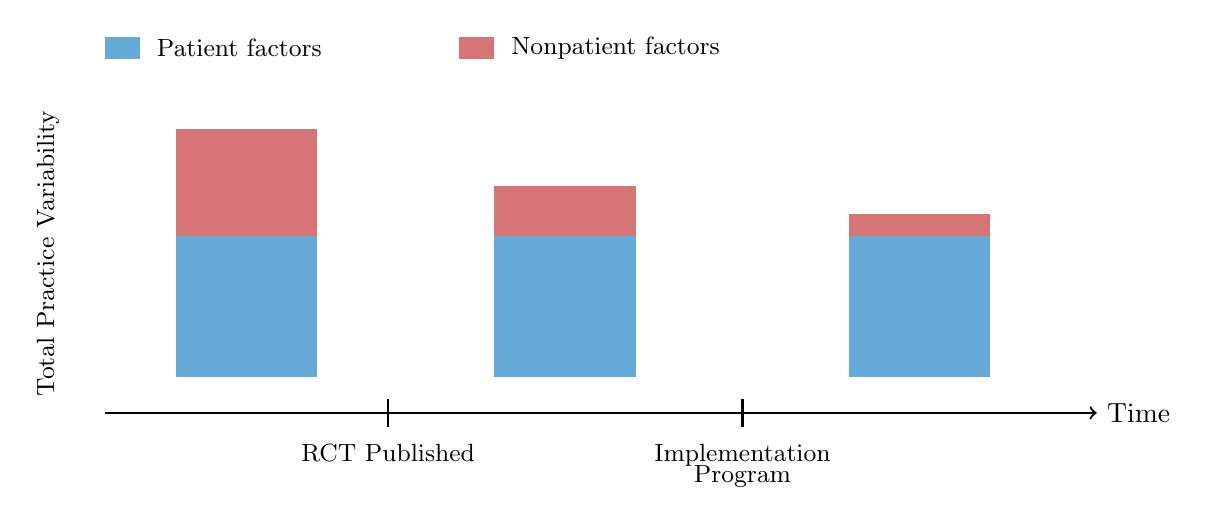
\begin{tikzpicture}[scale=0.9]
    % Timeline
    \draw[->, thick] (0,0) -- (14,0) node[right] {Time};

    % Markers
    \draw[thick] (4,-0.2) -- (4,0.2);
    \draw[thick] (9,-0.2) -- (9,0.2);

    % Labels
    \node[below] at (4,-0.3) {\small RCT Published};
    \node[below] at (9,-0.3) {\small Implementation};
    \node[below] at (9,-0.6) {\small Program};

    % Variability bars - Before RCT
    \fill[emergency_blue!60] (1,0.5) rectangle (3,2.5);
    \fill[emergency_red!60] (1,2.5) rectangle (3,4);

    % Variability bars - After RCT
    \fill[emergency_blue!60] (5.5,0.5) rectangle (7.5,2.5);
    \fill[emergency_red!60] (5.5,2.5) rectangle (7.5,3.2);

    % Variability bars - After Implementation
    \fill[emergency_blue!60] (10.5,0.5) rectangle (12.5,2.5);
    \fill[emergency_red!60] (10.5,2.5) rectangle (12.5,2.8);

    % Legend
    \fill[emergency_blue!60] (0,5) rectangle (0.5,5.3);
    \node[right] at (0.6,5.15) {\small Patient factors};
    \fill[emergency_red!60] (5,5) rectangle (5.5,5.3);
    \node[right] at (5.6,5.15) {\small Nonpatient factors};

    % Y-axis label
    \node[rotate=90] at (-0.8,2.25) {\small Total Practice Variability};
\end{tikzpicture}
\end{center}

\textbf{重點：}
\begin{enumerate}
    \item RCT 提供高品質證據 → 理想上減少 nonpatient factor 變異
    \item Implementation program → 進一步減少 nonpatient factor 變異
    \item Patient factor 變異維持不變（假設 case mix 不變）
\end{enumerate}

%============================================================
\section{Multilevel Modeling 的應用}
%============================================================

\subsection{什麼是 Multilevel Modeling？}

Multilevel modeling（多層次模型/階層模型）是一種統計方法，可處理具有巢狀結構的資料，例如：

\begin{center}
\textbf{病人} $\subset$ \textbf{醫師} $\subset$ \textbf{ICU} $\subset$ \textbf{醫院}
\end{center}

此方法可量化各層級對總變異的貢獻比例。

\subsection{Variance Partition Coefficient (VPC)}

VPC 定義為某層級變異佔總變異的比例：

\begin{equation}
\text{VPC} = \frac{\tau^2}{\tau^2 + \sigma^2}
\end{equation}

其中：
\begin{itemize}
    \item $\tau^2$ = 醫院層級（或其他層級）的變異
    \item $\sigma^2$ = 病人層級的變異（已調整病人特徵後）
\end{itemize}

\subsection{應用一：聚焦 Determinants of Practice 的搜尋}

\begin{tcolorbox}[colback=highlight_yellow,colframe=emergency_red,title=\textbf{假設範例}]
假設 multilevel modeling 分析顯示 EBP adoption 的變異來源：
\begin{itemize}[nosep]
    \item Hospital level: 6\%
    \item ICU level: \textbf{60\%}
    \item Clinician level: 9\%
    \item Patient case mix: 25\%
\end{itemize}

\textbf{結論：}Implementation program 應主要針對 \textbf{ICU 層級}的決定因素，因為這是最大的變異來源（60\%）。
\end{tcolorbox}

\subsection{應用二：評估 Implementation Program 的成效}

比較 implementation program 前後的 VPC：

\begin{longtable}{lcc}
\toprule
\textbf{變異來源} & \textbf{介入前} & \textbf{介入後} \\
\midrule
\endfirsthead
\bottomrule
\endfoot

Hospital & 6\% & 6\% \\
ICU & 60\% & 15\% \\
Clinicians & 9\% & 5\% \\
\midrule
\textbf{Nonpatient factors total} & \textbf{75\%} & \textbf{26\%} \\
\midrule
Patient case mix & 25\% & 74\% \\
\bottomrule
\end{longtable}

\textbf{結果：}Nonpatient factors 造成的變異從 75\% 降至 26\%，相對減少 \textbf{65\%}。

%============================================================
\section{LOTUS-FRUIT 研究的實證分析}
%============================================================

\subsection{研究背景}

LOTUS-FRUIT（Low Tidal Volume Universal Support: Feasibility of Recruitment for Interventional Trials）是由 Prevention and Early Treatment of Acute Lung Injury Network 進行的觀察性研究。

\textbf{研究假設：}
\begin{itemize}
    \item 2000 年 LTVV 被證實可改善 ARDS 病人存活率，成為 established EBP
    \item 但 LTVV 對非 ARDS 的 ARF（acute respiratory failure）病人效果較不明確
    \item 因此假設：ARDS 病人的 LTVV 使用變異應小於非 ARDS 病人
\end{itemize}

\subsection{研究方法}

\begin{longtable}{p{4cm}p{10cm}}
\toprule
\textbf{項目} & \textbf{內容} \\
\midrule
\endfirsthead
\bottomrule
\endfoot

資料來源 & LOTUS-FRUIT cohort study (2017) \\
\midrule
研究對象 & 45 家醫院、1,113 位病人、2,090 次觀察 \\
\midrule
ARDS 定義 & PaO$_2$/FiO$_2$ $\leq$ 300 mmHg + 雙側浸潤（24 小時內 CXR 確認）\\
\midrule
LTVV 定義 & 任一記錄的 tidal volume < 6.5 mL/kg predicted body weight \\
\midrule
統計模型 & Multilevel logistic regression with hospital-level random effect \\
\midrule
校正變項 & 年齡、性別、intubation indication、SOFA score（插管後 24 小時）\\
\bottomrule
\end{longtable}

\subsection{主要結果}

\begin{longtable}{p{4cm}ccc}
\caption{LOTUS-FRUIT 研究結果：LTVV 的 Variance Partition Coefficients} \\
\toprule
\textbf{分析} & \textbf{ARDS VPC} & \textbf{Non-ARDS VPC} & \textbf{相對差異} \\
\midrule
\endfirsthead

\toprule
\textbf{分析} & \textbf{ARDS VPC} & \textbf{Non-ARDS VPC} & \textbf{相對差異} \\
\midrule
\endhead

\bottomrule
\endfoot

Primary analysis\newline (n=1,113) & 20\%\newline (95\% CI: 13-35\%) & 34\%\newline (95\% CI: 24-58\%) & \textbf{41\% decrease} \\
\midrule
Sensitivity 1\newline (imputed ARDS) & 21\%\newline (95\% CI: 14-36\%) & 38\%\newline (95\% CI: 28-55\%) & \textbf{45\% decrease} \\
\midrule
Sensitivity 2\newline (day 0 data included) & 22\%\newline (95\% CI: 15-35\%) & 35\%\newline (95\% CI: 25-49\%) & \textbf{37\% decrease} \\
\midrule
Sensitivity 3\newline (LTVV < 8.0 mL/kg) & 21\%\newline (95\% CI: 15-47\%) & 25\%\newline (95\% CI: 16-43\%) & 16\% decrease \\
\bottomrule
\end{longtable}

\subsection{結果解讀}

\begin{tcolorbox}[colback=emergency_blue!5!white,colframe=emergency_blue,title=\textbf{重點解讀}]
\begin{enumerate}
    \item \textbf{ARDS 病人的 VPC 較低（20\% vs 34\%）：}符合假設——當 LTVV 為 established EBP 時，醫院間變異較小

    \item \textbf{20\% 的意涵：}約五分之一的 LTVV 使用變異來自非病人因素，是 implementation program 可改善的空間

    \item \textbf{< 8.0 mL/kg 閾值的結果：}ARDS 與非 ARDS 病人的 VPC 相近（21\% vs 25\%），顯示此閾值已被廣泛接受於所有機械通氣病人

    \item \textbf{期望管理：}若 implementation program 將 nonpatient factor 變異減半（20\% → 10\%），對整體 LTVV 使用率的影響可能仍然有限，因為 80\% 變異來自病人因素
\end{enumerate}
\end{tcolorbox}

%============================================================
\section{方法學限制與注意事項}
%============================================================

\subsection{量化分析無法回答的問題}

\begin{enumerate}
    \item \textbf{無法解釋「為什麼」：}
    \begin{itemize}
        \item 量化分析可指出變異主要在 ICU 層級
        \item 但無法說明是哪些 CFIR constructs 造成變異
        \item 仍需質性研究（訪談、觀察）來發掘具體原因
    \end{itemize}

    \item \textbf{決策歸屬的複雜性：}
    \begin{itemize}
        \item 部分病人可能在 ICU 外插管
        \item Team medicine 情境下，EMR 記錄的 order 可能是團隊討論結果
    \end{itemize}

    \item \textbf{Unmeasured confounders：}
    \begin{itemize}
        \item 本分析僅納入有限的病人變項
        \item 未測量的決定因素可能影響 VPC 估計
        \item 比較介入前後 VPC 時，需假設 unmeasured determinants 的影響維持恆定
    \end{itemize}
\end{enumerate}

\subsection{技術考量}

\begin{itemize}
    \item 使用 latent response formulation 將 within 與 between hospital variance 轉換至相同尺度
    \item Bootstrap method（1,000 samples）估計 VPC 差異的 confidence interval
    \item 當目標是量化各層級變異貢獻時，遺漏 unmeasured determinants 不會 bias VPC 估計
\end{itemize}

%============================================================
\section{臨床實務建議}
%============================================================

\begin{tcolorbox}[colback=emergency_blue!5!white,colframe=emergency_blue,title=\textbf{Implementation Science 實務應用}]

\textbf{Phase I：量化評估}
\begin{enumerate}
    \item 使用 multilevel modeling 分析現有觀察性資料
    \item 量化各層級（醫院、ICU、醫師、病人）對 EBP adoption 變異的貢獻
    \item 決定 implementation program 應聚焦的層級
\end{enumerate}

\textbf{Phase II：質性探索}
\begin{enumerate}
    \item 根據 Phase I 結果，聚焦於主要變異來源層級
    \item 使用 CFIR 框架進行訪談、問卷
    \item 識別該層級的具體 facilitators 與 barriers
\end{enumerate}

\textbf{Intervention Phase：}
\begin{enumerate}
    \item 設計針對性的 implementation program
    \item 納入標準的 process monitoring 與 evaluation
\end{enumerate}

\textbf{Evaluation Phase：}
\begin{enumerate}
    \item 重新計算 VPC
    \item 比較介入前後 nonpatient factor 變異的變化
    \item 可與其他 implementation strategies 進行比較
\end{enumerate}
\end{tcolorbox}

%============================================================
\section{結論}
%============================================================

\begin{enumerate}
    \item \textcolor{red}{\textbf{結論一：}}Practice variability 可透過 multilevel modeling 量化，區分為 patient factors 與 nonpatient factors 兩大來源。

    \item \textcolor{red}{\textbf{結論二：}}VPC 可指導 implementation program 聚焦於最大變異來源，提高介入效率。

    \item \textcolor{red}{\textbf{結論三：}}LOTUS-FRUIT 資料證實：當 EBP 有強證據支持時（ARDS + LTVV），醫院間變異較小（VPC 20\% vs 34\%）。

    \item \textcolor{red}{\textbf{結論四：}}量化方法應與質性研究（如 CFIR）互補，而非取代。

    \item \textcolor{red}{\textbf{結論五：}}此方法也可用於評估 implementation program 成效，並比較不同 implementation strategies。
\end{enumerate}

\vspace{0.5cm}
\textbf{關鍵詞：}Implementation Science、Practice Variability、Multilevel Modeling、CFIR、Low-Tidal Volume Ventilation、ARDS、Variance Partition Coefficient

%============================================================
\section{參考文獻}
%============================================================

\begin{enumerate}
    \item Turnbull AE, Zhang S, Colantuoni E, et al. Quantifying Practice Variability to Inform the Design of Implementation Programs in Critical Care and Assess Their Impact. \href{https://doi.org/10.1016/j.chest.2025.08.026}{\textit{CHEST}. 2026;169(1):128-138.}

    \item Damschroder LJ, Reardon CM, Widerquist MAO, Lowery J. The updated Consolidated Framework for Implementation Research based on user feedback. \href{https://doi.org/10.1186/s13012-022-01245-0}{\textit{Implement Sci}. 2022;17(1):75.}

    \item The ARDS Network. Ventilation with lower tidal volumes as compared with traditional tidal volumes for acute lung injury and the acute respiratory distress syndrome. \href{https://doi.org/10.1056/NEJM200005043421801}{\textit{N Engl J Med}. 2000;342(18):1301-1308.}

    \item Lanspa MJ, Gong MN, Schoenfeld DA, et al. Prospective assessment of the feasibility of a trial of low-tidal volume ventilation for patients with acute respiratory failure. \href{https://doi.org/10.1513/AnnalsATS.201809-627OC}{\textit{Ann Am Thorac Soc}. 2019;16(3):356-362.}

    \item Fan E, Del Sorbo L, Goligher EC, et al. An Official American Thoracic Society/European Society of Intensive Care Medicine/Society of Critical Care Medicine Clinical Practice Guideline: mechanical ventilation in adult patients with acute respiratory distress syndrome. \href{https://doi.org/10.1164/rccm.201703-0548ST}{\textit{Am J Respir Crit Care Med}. 2017;195(9):1253-1263.}

    \item Bellani G, Laffey JG, Pham T, et al. Epidemiology, patterns of care, and mortality for patients with acute respiratory distress syndrome in intensive care units in 50 countries. \href{https://doi.org/10.1001/jama.2016.0291}{\textit{JAMA}. 2016;315(8):788-800.}
\end{enumerate}

%============================================================
\section{縮寫對照表}
%============================================================

\begin{longtable}{p{4cm}p{10cm}}
\toprule
\textbf{縮寫} & \textbf{全名} \\
\midrule
\endfirsthead

\toprule
\textbf{縮寫} & \textbf{全名} \\
\midrule
\endhead

\bottomrule
\endfoot

ARDS & Acute Respiratory Distress Syndrome (急性呼吸窘迫症候群) \\
ARF & Acute Respiratory Failure (急性呼吸衰竭) \\
CFIR & Consolidated Framework for Implementation Research (實施研究整合框架) \\
CI & Confidence Interval (信賴區間) \\
EBP & Evidence-Based Practice (實證醫學實務) \\
LOTUS-FRUIT & Low Tidal Volume Universal Support: Feasibility of Recruitment for Interventional Trials \\
LTVV & Low-Tidal Volume Ventilation (低潮氣容積通氣) \\
PBW & Predicted Body Weight (預測體重) \\
SOFA & Sequential Organ Failure Assessment (連續性器官衰竭評估) \\
VPC & Variance Partition Coefficient (變異分割係數) \\
\bottomrule
\end{longtable}

\end{document}
